\documentclass{ximera}

\newcommand{\RR}{\mathbb R}
\renewcommand{\d}{\,d}
\newcommand{\dd}[2][]{\frac{d #1}{d #2}}
\renewcommand{\l}{\ell}
\newcommand{\ddx}{\frac{d}{dx}}
\newcommand{\dfn}{\textbf}
\newcommand{\eval}[1]{\bigg[ #1 \bigg]}


\author{Bart Snapp}

\begin{document}

\begin{problem}
  Sketch the region of integration for the integral: $\int_0^\pi
  \int_y^\pi \frac{\sin(x)}{x}\d x \d y$
  \begin{image}[2in]
    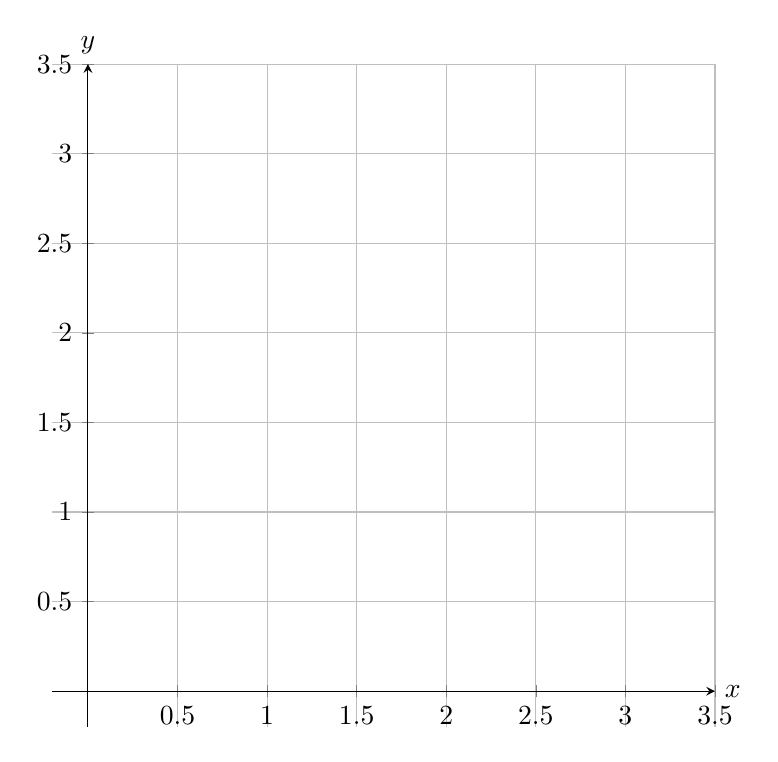
\begin{tikzpicture}
      \begin{axis}[
          xmin=-.2, xmax=3.5,ymin=-.2,ymax=3.5,
          clip=false,
          axis lines=center,
          width=10cm,
          height=10cm,
          xtick={0,.5,...,3.5},
          ytick={0,.5,...,3.5},
          xlabel=$x$, ylabel=$y$,
          grid = major,
          every axis y label/.style={at=(current axis.above origin),anchor=south},
          every axis x label/.style={at=(current axis.right of origin),anchor=west},
        ]
        %\addplot[very thick,black,->] plot coordinates {(1,1) (4,2)};
        %\addplot[very thick,black,->] plot coordinates {(-1,0) (-3,3)};
        %\node[above] at (axis cs:2.5, 1.5) {$\vec{w}$};
        %\node[above] at (axis cs:-2, 1.5) {$\vec{v}$};
      \end{axis}
    \end{tikzpicture}
  \end{image}
    \begin{prompt}
    \begin{multipleChoice}
        \choice[correct]{I've drawn this.}
    \end{multipleChoice}
    \begin{feedback}[correct]
        \begin{image}
          \includegraphics{scan2.jpg}
        \end{image}
      \end{feedback}
    \end{prompt}
\end{problem}

\begin{problem}
  Compute the integral: $\int_0^\pi \int_y^\pi \frac{\sin(x)}{x}\d x \d y$
  \begin{prompt}
    \[
    =\answer{2}
    \]
  \end{prompt}
  \vfill
\end{problem}

\begin{problem}
  Suppose $f:\R\to\R$ is a function with the property that:
  \[
  \int_0^4 f(t) \d t = \pi
  \]
  Let $C = \{(x,y): x^2+y^2 \le 4\}$. Compute:
  \[
  \iint_C f(x^2 + y^2) \d A
  \begin{prompt}
    = \answer{\pi^2}
      \end{prompt}
  \]
  \vfill
\end{problem}
\end{document}
